\documentclass{article}

\usepackage{geometry}
    \geometry{top=5mm}
    \geometry{left=5mm}
    \geometry{right=5mm}
    \geometry{bottom=5mm}
    
\usepackage{tikz}
\usetikzlibrary{automata, positioning}

\begin{document}
\centering
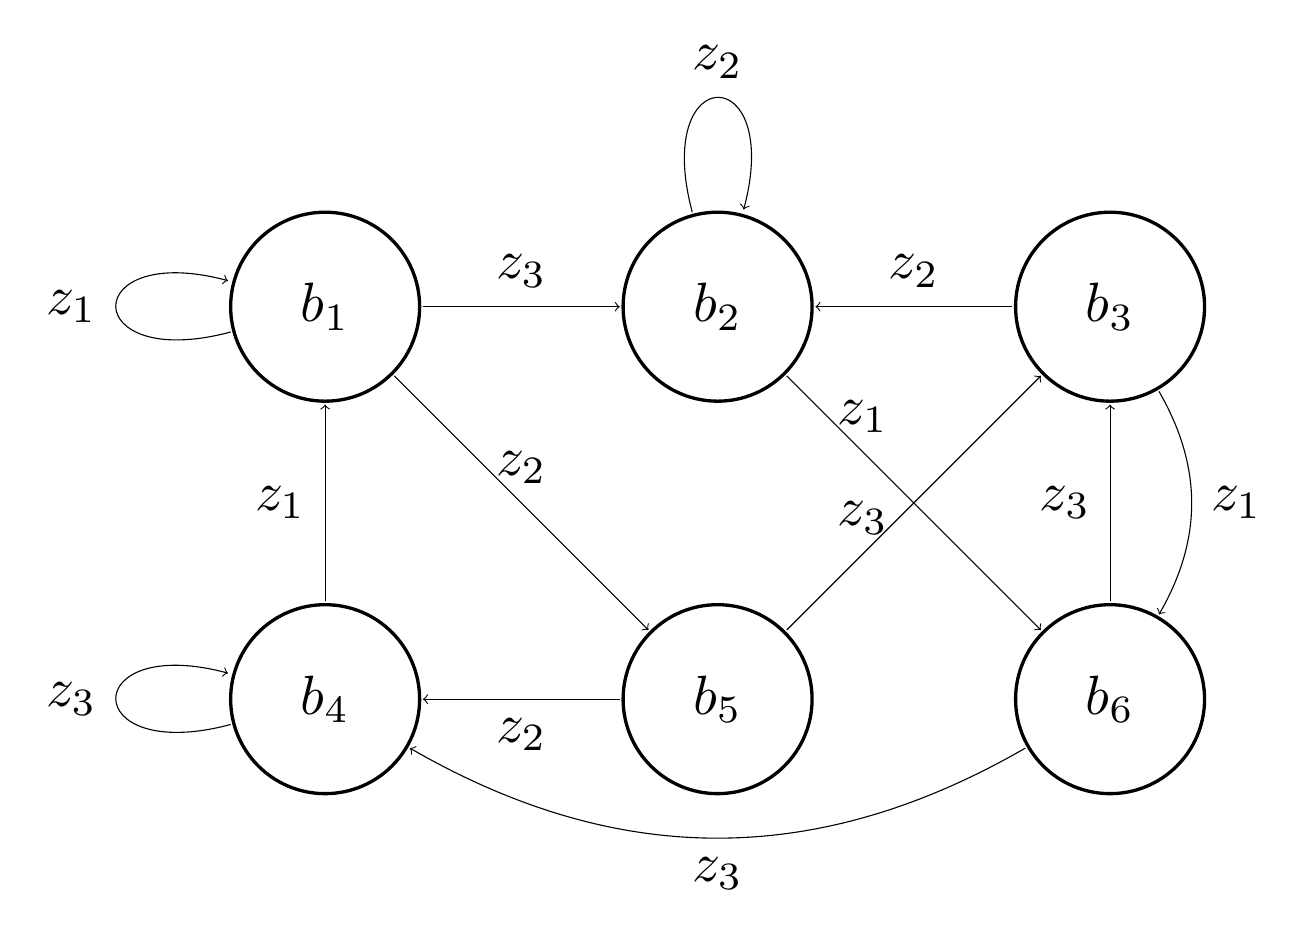
\begin{tikzpicture}[
roundnode/.style={circle, draw=black, very thick, minimum size=12mm},
every node/.style={scale=2},
scale=2
]

\node[roundnode] (circle_b1) {$b_1$};
\node[roundnode] (circle_b2) [right=2.5cmof circle_b1] {$b_2$};
\node[roundnode] (circle_b3) [right=2.5cmof circle_b2] {$b_3$};
\node[roundnode] (circle_b4) [below=2.5cmof circle_b1] {$b_4$};
\node[roundnode] (circle_b5) [right=2.5cmof circle_b4] {$b_5$};
\node[roundnode] (circle_b6) [right=2.5cmof circle_b5] {$b_6$};

\path[->] (circle_b1) edge node [pos=0.5, above] {$z_3$} (circle_b2);
\path[->] (circle_b1) edge node [pos=0.5, above] {$z_2$} (circle_b5); 
\path[->] (circle_b1) edge [loop left] node {$z_1$} (circle_b1);

\path[->] (circle_b2) edge [loop above] node {$z_2$} (circle_b2);
\path[->] (circle_b2) edge node [pos=0.3, above] {$z_1$} (circle_b6);

\path[->] (circle_b3) edge node [pos=0.5, above] {$z_2$} (circle_b2); 
\path[->] (circle_b3) edge [bend left] node [pos=0.5, right] {$z_1$} (circle_b6);

\path[->] (circle_b4) edge node [pos=0.5, left] {$z_1$} (circle_b1);
\path[->] (circle_b4) edge [loop left] node {$z_3$} (circle_b4);

\path[->] (circle_b5) edge node [pos=0.5, below] {$z_2$} (circle_b4);
\path[->] (circle_b5) edge node [pos=0.3, above] {$z_3$} (circle_b3);

\path[->] (circle_b6) edge [bend left] node [pos=0.5, below] {$z_3$} (circle_b4);
\path[->] (circle_b6) edge node [pos=0.5, left] {$z_3$} (circle_b3);

\end{tikzpicture}
\end{document}